\documentclass[10pt, t,
%aspectratio=169,% for widescreen (16:9) presentations
aspectratio=1610,% for (16:10) presentations
%aspectratio=43,% for traditional (4:3) presentations
% handout%
usenames,
dvipsnames,
]{beamer}

\usetheme{Berkeley}

\usepackage{default}
\usepackage{xcolor}
\usepackage{xspace}
\usepackage{algorithm}
\usepackage[noend]{algpseudocode}
\usepackage{listings}
\usepackage{tikz}
\usetikzlibrary{arrows,
	petri,
	topaths,
	calc,
	positioning,
	automata,
}
\usepackage{siunitx}
\usepackage{diagbox}
\usepackage{tikz-network}
\usepackage{bibentry}

\bibliographystyle{apalike}

% add the following two lines to your document to get bigger arrows
\usetikzlibrary{arrows.meta}
\tikzset{>={Latex[width=3mm,length=3mm]}}

\newcommand{\TODO}[1]{\noindent\textcolor{green}{\textbf{TODO:} #1}}

\newcommand{\pathfinder}{\textsc{Pathfinder}\xspace}
\newcommand{\findEdgeCandidates}{FindEdgeCandidates\xspace}
\newcommand{\refineEdgeCandidates}{RefineEdgeCandidates\xspace}
\newcommand{\getAssociatedTrajectories}{GetAssociatedTrajectories\xspace}

\newcommand{\chrep}{CH-representation\xspace}

\newcommand{\traj}[2]{\mathcal{T}_{\text{#1},\text{#2}}}

\title[Pathfinder] % (optional, only for long titles)
{PATHFINDER}
\subtitle{Storage and Indexing of Massive Trajectory Sets}
\author[Funke, Nusser, Rupp, Storandt] % (optional, for multiple authors)
{Stefan~Funke\inst{1} \and Andr\'{e}~Nusser\inst{2} \and Tobias~Rupp\inst{3} \and Sabine~Storandt\inst{4}}
\institute[Universities] % (optional)
{
	\inst{1}%
	University of Stuttgart
	\and
	\inst{2}%
	Max Planck Institute for Informatics
	\and
	\inst{3}%
	University of Stuttgart
	\and
	\inst{4}%
	University of Konstanz
}
\date[SSTD 2019] % (optional)
{SSTD, 2019}
\subject{Computer Science}


\begin{document}
\frame{\titlepage}
\nobibliography{vldb}  % vldb_sample.bib is the name of the Bibliography in this case

\section{Motivation}
\begin{frame}
	\frametitle{Motivation}
	\begin{minipage}[t]{0.45\textwidth}
		\vspace{0pt}
		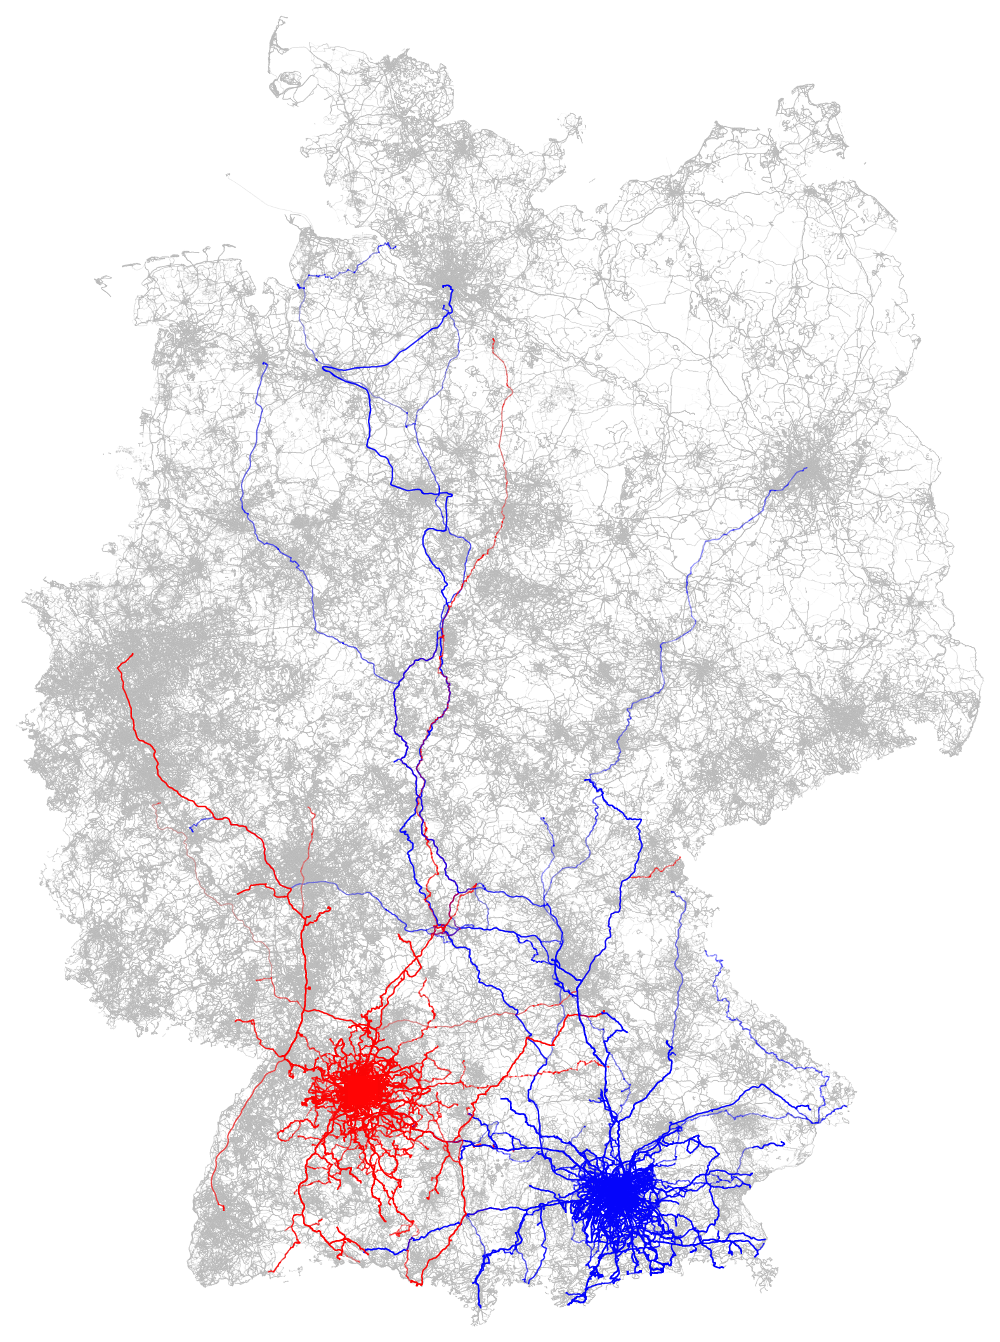
\includegraphics[height=0.9\textheight]{images/trajectories.png}
	\end{minipage}
	\hfill
	\begin{minipage}[t]{0.45\textwidth}
		\vspace{0pt}
		\begin{itemize}
			\item<1->plenty of devices capable of tracking positions
			\item<2-> huge and growing volume of trajectory data
			\item<3-> often no efficient retrieval
			\item<4-> applications:
			      \begin{itemize}
				      \item<5-> analysis of commute patterns
				      \item<6-> traffic flow estimation/prediction
				      \item<7-> traffic infrastructure planning
				      \item<8-> proposal of hiking routes
			      \end{itemize}

		\end{itemize}
	\end{minipage}
\end{frame}

\section{Problem Description}
\begin{frame}
	\frametitle{Problem Description}
	\begin{minipage}[t]{0.45\textwidth}
		\vspace{0pt}
		\includegraphics<1>[keepaspectratio,height=1.2\textheight,width=1.2\textwidth]{graphics/saarland_real_data/saarland_real_data_1.png}
		\includegraphics<2-4>[keepaspectratio,height=1.2\textheight,width=1.2\textwidth]{graphics/saarland_real_data/saarland_real_data_2.png}
		\includegraphics<5>[keepaspectratio,height=1.2\textheight,width=1.2\textwidth]{graphics/saarland_real_data/saarland_real_data_3.png}
		\includegraphics<6>[keepaspectratio,height=1.2\textheight,width=1.2\textwidth]{graphics/saarland_real_data/saarland_real_data_4.png}
	\end{minipage}
	\hfill
	\begin{minipage}[t]{0.45\textwidth}
		\vspace{0pt}
		\begin{itemize}
			\item road network graph $G(V,E,c)$ \pause
			\item map-matched trajectories \pause

			      (map-matching: fit raw gps-positions on network graph)\pause

			      $\Rightarrow$ 1.Problem: \textbf{Compression} \pause
			\item \emph{window}-query \pause

			      $\Rightarrow$ 2.Problem: \textbf{Retrieval} of intersecting trajectories
		\end{itemize}
	\end{minipage}
\end{frame}

\section{Contribution}
\begin{frame}
	\frametitle{Contribution}
	\begin{itemize}
		\item novel data structure \pathfinder \pause
		      \begin{itemize}
			      \item compressing and storing large-scale trajectory data \pause

			            (hundreds of millions of trajectories) \pause
			      \item efficient retrieval from this data \pause

			            (~5 ns per reported trajectory)
		      \end{itemize}
	\end{itemize}
\end{frame}


\section{Contraction Hierarchies}

\begin{frame}{Contraction Hierarchies}
	\begin{itemize}[<+(1)->]
		\item basis data structure of \pathfinder
		\item data structure to speed up shortest-path queries (ms $\rightarrow$ s) \cite{Geisberger:ch}
		\item augmentation of the original graph $G$
	\end{itemize}
\end{frame}

\begin{frame}{Contraction Hierarchies}
	\framesubtitle{Construction}
	\begin{itemize}[<+(1)->]
		\item remove nodes one-by-one
		\item order can be arbitrary and defines levels
		\item add \emph{shortcut} edges to retain shortest paths
		\item original graph + all \emph{shortcut} edges ever created = CH
		\item construction time is typically several minutes and \#shortcuts $<$ \#original edges
	\end{itemize}
\end{frame}

\begin{frame}{Contraction Hierarchies}
	\framesubtitle{Construction (Example - remove node $v$)}
	\centering
	\includegraphics<2>[keepaspectratio,height=.8\textheight,width=.8\textwidth]{graphics/ch_constr/ch_constr_1.eps}%
	\includegraphics<3>[keepaspectratio,height=.8\textheight,width=.8\textwidth]{graphics/ch_constr/ch_constr_2.eps}%
	\includegraphics<4>[keepaspectratio,height=.8\textheight,width=.8\textwidth]{graphics/ch_constr/ch_constr_3.eps}%
\end{frame}

\section{Compression}

\begin{frame}
	\frametitle{Compression}
	\framesubtitle{\chrep}
	\begin{minipage}[t]{0.45\textwidth}
		\vspace{0pt}
		\resizebox{\textwidth}{!}{
			\begin{tikzpicture}

				\tikzset{VertexStyle/.style =
						{shape=circle, fill=black, minimum size = 0pt,inner sep=0pt}
				}
				\Vertex[x=-1, y=-2]{origin}

				%level axis
				\Vertex[x=-1, y=3, label=level, position=left]{level_u}
				\Edge[Direct, lw=1pt](origin)(level_u)

				%x-axis
				\Vertex[x=6, y=-2, label=x, position=below]{x_u}
				\Edge[Direct, lw=1pt](origin)(x_u)

				\tikzset{VertexStyle/.style =
						{shape=circle, fill=black, minimum size = 4pt,inner sep=0pt}
				}
				\Vertex[x=0,y=1, label=1, position=below]{1}
				\Vertex[x=2,y=-1, label=2, position=below]{2}
				\Vertex[x=3,y=3, label=3, position=below]{3}
				\Vertex[x=4,y=1, label=4, position=below]{4}
				\Vertex[x=5,y=0, label=5, position=below]{5}
				\Vertex[x=6,y=2, label=6, position=below]{6}

				\tikzstyle{EdgeStyle}=[color=red]

				%original
				\only<1>{
					\Edge(1)(2)
				}
				\only<2,6->{
					\Edge[style=dashed](1)(2)
				}

				\only<1>{
					\Edge(2)(3)
				}
				\only<2,6->{
					\Edge[style=dashed](2)(3)
				}

				\only<1-3>{
					\Edge(3)(4)
				}
				\only<4,6->{
					\Edge[style=dashed](3)(4)
				}

				\only<1-2>{
					\Edge(4)(5)
				}
				\only<3,6->{
					\Edge[style=dashed](4)(5)
				}

				\only<1-2>{
					\Edge(5)(6)
				}
				\only<3,6->{
					\Edge[style=dashed](5)(6)
				}

				%shortcuts
				\only<2->{
					\Edge(1)(3)
				}

				\only<3>{
					\Edge(4)(6)
				}
				\only<4>{
					\Edge[style=dashed](4)(6)
				}

				\only<4->{
					\Edge(3)(6)
				}
			\end{tikzpicture}
		}
	\end{minipage}
	\hfill
	\begin{minipage}[t]{0.45\textwidth}
		\vspace{0pt}
		\begin{itemize}
			\item<2-> Substitute edges with shortcuts
			\item<6-> Reverse substitution to decompress
			\item<7-> experiments: compression ratio 10
		\end{itemize}
	\end{minipage}
\end{frame}

\section{Retrieval}

\begin{frame}
	\frametitle{Retrieval Overview}
	\begin{minipage}[t]{0.45\textwidth}
		\vspace{0pt}
		\includegraphics<1-2,5>[keepaspectratio,height=1.2\textheight,width=1.2\textwidth]{graphics/saarland_real_data/saarland_real_data_4.png}
		\includegraphics<3>[keepaspectratio,height=1.2\textheight,width=1.2\textwidth]{graphics/saarland_real_data/saarland_real_data_3.png}
		\includegraphics<4>[keepaspectratio,height=1.2\textheight,width=1.2\textwidth]{graphics/saarland_real_data/saarland_real_data_edgesInRectangle.png}
	\end{minipage}
	\hfill
	\begin{minipage}[t]{0.45\textwidth}
		\vspace{0pt}
		\begin{itemize}
			\item<2-> Naive way: Check all trajectories\pause
			\item<3-> Inverted Index:
			      \begin{enumerate}
				      \item<4-> Collect edges within rectangle \pause
				      \item<5-> Report all associated trajectories \pause
			      \end{enumerate}
		\end{itemize}
	\end{minipage}
\end{frame}

\begin{frame}
	\frametitle{Inverted Index}
	\framesubtitle{Edge Association}
	\begin{minipage}[t]{0.45\textwidth}
		\vspace{0pt}
		\resizebox{\textwidth}{!}{
			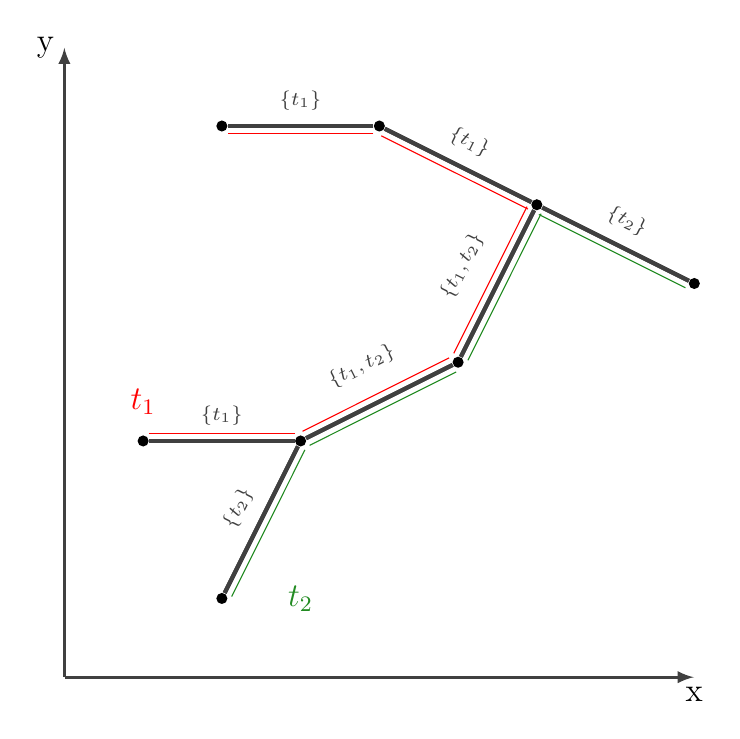
\begin{tikzpicture}

				%axes
				\tikzset{VertexStyle/.style =
						{shape=circle, fill=black, minimum size = 0pt,inner sep=0pt}
				}

				\Vertex[x=1, y=1]{origin}

				%x-axis
				\Vertex[x=9, y=1, label=x, position=below, fontsize=\large]{x_u}
				\Edge[Direct, lw=1pt](origin)(x_u)

				%y-axis
				\Vertex[x=1, y=9, label=y, position=left, fontsize=\large]{y_u}
				\Edge[Direct, lw=1pt](origin)(y_u)

				\tikzset{VertexStyle/.style =
						{shape=circle, fill=black, minimum size = 4pt,inner sep=0pt}
				}
				\Vertex[x=2,y=4]{1}
				\Vertex[x=3,y=2]{2}
				\Vertex[x=4,y=4]{3}
				\Vertex[x=6,y=5]{4}
				\Vertex[x=7,y=7]{5}
				\Vertex[x=9,y=6]{6}
				\Vertex[x=5,y=8]{7}
				\Vertex[x=3,y=8]{8}


				%graph edges
				\Edge(1)(3)
				\Edge(2)(3)
				\Edge(3)(4)
				\Edge(4)(5)
				\Edge(5)(6)
				\Edge(5)(7)
				\Edge(7)(8)

				\tikzset{VertexStyle/.style =
						{minimum size = 0pt,inner sep=0pt}
				}

				%t_1
				\Vertex[x=2,y=4.5, label=$t_1$, fontcolor=red, fontsize=\large]{redLabel}

				\tikzset{auto shift/.style={auto=left,
				to path={ let \p1=(\tikztostart),\p2=(\tikztotarget),
				\n1={atan2(\y2-\y1,\x2-\x1)},\n2={\n1+180}
				in ($(\tikztostart.{\n1})!1mm!90:(\tikztotarget.{\n2})$) --
				($(\tikztotarget.{\n2})!1mm!270:(\tikztostart.{\n1})$) \tikztonodes}}}

				\draw
				(1) edge[auto shift, color=red] (3)
				(3) edge[auto shift, color=red] (4)
				(4) edge[auto shift, color=red] (5)
				(5) edge[auto shift, color=red] (7)
				(7) edge[auto shift, color=red] (8)
				;

				%t_2
				\Vertex[x=4,y=2, label=$t_2$, fontcolor=ForestGreen, fontsize=\large]{greenLabel}

				\tikzset{auto shift/.style={auto=right,
				to path={ let \p1=(\tikztostart),\p2=(\tikztotarget),
				\n1={atan2(\y2-\y1,\x2-\x1)},\n2={\n1+180}
				in ($(\tikztostart.{\n1})!1mm!270:(\tikztotarget.{\n2})$) --
				($(\tikztotarget.{\n2})!1mm!90:(\tikztostart.{\n1})$) \tikztonodes}}}

				\draw
				(2) edge[auto shift, color=ForestGreen] (3)
				(3) edge[auto shift, color=ForestGreen] (4)
				(4) edge[auto shift, color=ForestGreen] (5)
				(5) edge[auto shift, color=ForestGreen] (6)
				;

				\only<3->{
					//labeled edges, draw them over the old ones
					\Edge[label={$\{t_1\}$}, position=above, style={sloped}](1)(3)
					\Edge[label={$\{t_2\}$}, position=above, style={sloped}](2)(3)
					\Edge[label={$\{t_1, t_2\}$}, position=above, style={sloped}](3)(4)
					\Edge[label={$\{t_1, t_2\}$}, position=above, style={sloped}](4)(5)
					\Edge[label={$\{t_2\}$}, position=above, style={sloped}](5)(6)
					\Edge[label={$\{t_1\}$}, position=above, style={sloped}](5)(7)
					\Edge[label={$\{t_1\}$}, position=above, style={sloped}](7)(8)
				}
			\end{tikzpicture}
		}
	\end{minipage}
	\hfill
	\begin{minipage}[t]{0.45\textwidth}
		\vspace{0pt}
		\begin{itemize}
			\item<2->associate trajectory with all its edges (pre-processing)
			\item<4->\chrep reduces associations
		\end{itemize}
	\end{minipage}
\end{frame}

\begin{frame}
	\frametitle{Collect edge candidates}

	\begin{minipage}[t]{0.45\textwidth}
		\vspace{0pt}

		\begin{tikzpicture}

			%\SetGraphUnit{1}

			%\GraphInit[vstyle=Classic]
			\tikzset{VertexStyle/.style =
					{shape=circle, fill=black, minimum size = 4pt,inner sep=0pt}
			}

			%edge
			\tikzstyle{EdgeStyle}=[->, color=black]
			\Vertex[x=-0.5,y=2]{source}
			\Vertex[x=1,y=3.25]{target}

			\Edge[label=e,position=above](source)(target) {e}


			\tikzset{VertexStyle/.style =
					{shape=circle, fill=black, minimum size = 0pt,inner sep=0pt}
			}

			\only<3-4>{
			%pathBox
			\Vertex[x=1.5,y=2]{6}
			\Vertex[x=1.5,y=3.25]{7}
			\Vertex[x=-0.5,y=3.25]{8}

			\tikzstyle{EdgeStyle}=[color=red]
			\Edge(source)(6)
			\Edge(6)(7)
			\Edge(7)(8)
			\Edge(8)(source)
			}

			%queryBox
			\Vertex[x=1.25,y=1.75]{1}
			\Vertex[x=3,y=1.75]{2}
			\Vertex[x=3,y=2.75]{3}
			\Vertex[x=1.25,y=2.75]{4}

			\tikzstyle{EdgeStyle}=[color=blue]
			\Edge(1)(2)
			\Edge[label=Q,position=right, fontcolor=blue](2)(3)
			\Edge(3)(4)
			\Edge(4)(1)

			%unpacked
			\tikzset{VertexStyle/.style =
					{shape=circle, fill=black, minimum size = 4pt,inner sep=0pt}
			}

			%possibility2
			\only<2-3>{
			\Vertex[x=1.5,y=2.5]{10}

			\tikzstyle{EdgeStyle}=[->, color=brown, dashed]
			\Edge(source)(10)
			\Edge(10)(target)
			}

		\end{tikzpicture}
	\end{minipage}
	\hfill
	\begin{minipage}[t]{0.45\textwidth}
		\vspace{0pt}
		\begin{itemize}
			\item<1-> Naive: Check intersection of edge with query rectangle
			\item<2-> But $e$ can represent an intersecting path!
			\item<3-> $\Rightarrow$ create path box($e$) in preprocessing
			\item<4-> $\Rightarrow$ fast check if $e$ is a candidate for intersection
		\end{itemize}
	\end{minipage}
\end{frame}

\begin{frame}
	\frametitle{Refine edge candidates}

	\begin{minipage}[t]{0.45\textwidth}
		\vspace{0pt}

		\begin{tikzpicture}

			%\SetGraphUnit{1}

			%\GraphInit[vstyle=Classic]
			\tikzset{VertexStyle/.style =
					{shape=circle, fill=black, minimum size = 4pt,inner sep=0pt}
			}

			%edge
			\tikzstyle{EdgeStyle}=[->, color=black]
			\Vertex[x=-0.5,y=2]{source}
			\Vertex[x=1,y=3.25]{target}

			\Edge[label=e,position=above](source)(target) {e}


			\tikzset{VertexStyle/.style =
					{shape=circle, fill=black, minimum size = 0pt,inner sep=0pt}
			}

			%pathBox
			\Vertex[x=1.5,y=2]{6}
			\Vertex[x=1.5,y=3.25]{7}
			\Vertex[x=-0.5,y=3.25]{8}

			\tikzstyle{EdgeStyle}=[color=red]
			\Edge(source)(6)
			\Edge(6)(7)
			\Edge(7)(8)
			\Edge(8)(source)

			%queryBox
			\Vertex[x=1.25,y=1.75]{1}
			\Vertex[x=3,y=1.75]{2}
			\Vertex[x=3,y=2.75]{3}
			\Vertex[x=1.25,y=2.75]{4}

			\tikzstyle{EdgeStyle}=[color=blue]
			\Edge(1)(2)
			\Edge[label=Q,position=right, fontcolor=blue](2)(3)
			\Edge(3)(4)
			\Edge(4)(1)

			%unpacked
			\tikzset{VertexStyle/.style =
					{shape=circle, fill=black, minimum size = 4pt,inner sep=0pt}
			}

			\only<4>{
			%possibility1
			\Vertex[x=1.5,y=3]{9}

			\tikzstyle{EdgeStyle}=[->, color=ForestGreen, dashed]
			\Edge(source)(9)
			\Edge(9)(target)
			}

			\only<3>{
			%possibility2
			\Vertex[x=1.5,y=2.5]{10}

			\tikzstyle{EdgeStyle}=[->, color=brown, dashed]
			\Edge(source)(10)
			\Edge(10)(target)
			}
		\end{tikzpicture}

		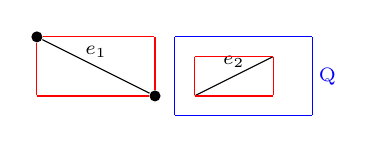
\begin{tikzpicture}
			\only<5>{
				%\SetGraphUnit{1}

				%\GraphInit[vstyle=Classic]
				\tikzset{VertexStyle/.style =
					{shape=circle, fill=black, minimum size = 4pt,inner sep=0pt}
			}

			%edge1
			\tikzstyle{EdgeStyle}=[->, color=black]
			\Vertex[x=1,y=2]{source}
			\Vertex[x=-0.5,y=2.75]{target}

			\Edge[label=$e_1$,position=above](source)(target) {e1}


			\tikzset{VertexStyle/.style =
					{shape=circle, fill=black, minimum size = 0pt,inner sep=0pt}
			}

			%pathBox1
			\Vertex[x=-0.5,y=2]{6}
			\Vertex[x=1,y=2.75]{8}

			\tikzstyle{EdgeStyle}=[color=red]
			\Edge(source)(6)
			\Edge(6)(target)
			\Edge(target)(8)
			\Edge(8)(source)

			%edge2
			\tikzstyle{EdgeStyle}=[->, color=black]
			\Vertex[x=1.5,y=2]{source}
			\Vertex[x=2.5,y=2.5]{target}

			\Edge[label=$e_2$,position=above](source)(target) {e2}

			%pathBox2
			\Vertex[x=1.5,y=2.5]{10}
			\Vertex[x=2.5,y=2]{12}

			\tikzstyle{EdgeStyle}=[color=red]
			\Edge(source)(10)
			\Edge(10)(target)
			\Edge(target)(12)
			\Edge(12)(source)

			%queryBox
			\tikzset{VertexStyle/.style =
					{shape=circle, fill=black, minimum size = 0pt,inner sep=0pt}
			}

			\Vertex[x=1.25,y=1.75]{1}
			\Vertex[x=3,y=1.75]{2}
			\Vertex[x=3,y=2.75]{3}
			\Vertex[x=1.25,y=2.75]{4}

			\tikzstyle{EdgeStyle}=[color=blue]
			\Edge(1)(2)
			\Edge[label=Q,position=right, fontcolor=blue](2)(3)
			\Edge(3)(4)
			\Edge(4)(1)
			}
		\end{tikzpicture}
	\end{minipage}
	\hfill
	\begin{minipage}[t]{0.45\textwidth}
		\vspace{0pt}
		\begin{itemize}
			\item<1-> $PB(e) \cap Q \neq \emptyset \Rightarrow e$ is candidate
			\item<2-> Which path does it bridge?
			      \begin{enumerate}
				      \item<3-> \textcolor{brown}{brown} path $\Rightarrow$ Accept candidate
				      \item<4-> \textcolor{ForestGreen}{green} path $\Rightarrow$ Reject candidate
			      \end{enumerate}
			\item<5-> no further inspection of non-intersecting path box necessary
		\end{itemize}
	\end{minipage}
\end{frame}

%\subsection{\getAssociatedTrajectories}
%\begin{frame}
%	\frametitle{\getAssociatedTrajectories}
%	Finally collect all trajectories associated with the remaining candidate edges, i.e. $t \in \bigcup_{e \in E_r} \mathcal{T}_e $.\pause
%
%	Removal of duplicates is also required, as trajectories are associated with more than one edge.
%\end{frame}

\section{Extensions}

\newcommand\interval[2]{
	%connection
	\draw let \p1 = (#1),\p2 = (#2) in
	(\x1,\y1) to (\x2,\y2);
	%left border
	\draw let \p1 = (#1),\p2 = (#2) in
	(\x1,\y1-5) to (\x1,\y1+5);
	%right border
	\draw let \p1 = (#1),\p2 = (#2) in
	(\x2,\y2-5) to (\x2,\y2+5);
}

\begin{frame}
	\frametitle{Extensions}
	\framesubtitle{Optimization: CH as R-Tree}
	\begin{minipage}[t]{0.45\textwidth}
		\vspace{0pt}
		\resizebox{\textwidth}{!}{
			\begin{tikzpicture}

				%level axis
				\tikzset{VertexStyle/.style =
						{shape=circle, fill=black, minimum size = 0pt,inner sep=0pt}
				}
				\Vertex[x=-1, y=-2]{origin}

				%level axis
				\Vertex[x=-1, y=3, label=level, position=left]{level_u}
				\Edge[Direct, lw=1pt](origin)(level_u)

				%x-axis
				\Vertex[x=6, y=-2, label=x, position=below]{x_u}
				\Edge[Direct, lw=1pt](origin)(x_u)

				\tikzset{VertexStyle/.style =
						{shape=circle, fill=black, minimum size = 4pt,inner sep=0pt}
				}
				\Vertex[x=0,y=1, label=1, position=below]{1}
				\Vertex[x=2,y=-1, label=2, position=below]{2}
				\Vertex[x=3,y=3, label=3, position=below]{3}
				\Vertex[x=4,y=1, label=4, position=below]{4}
				\Vertex[x=5,y=0, label=5, position=below]{5}
				\Vertex[x=6,y=2, label=6, position=below]{6}

				%original picture
				\tikzstyle{EdgeStyle}=[color=red]
				\only<1>{
					\Edge[style=dashed](1)(2)
					\Edge[style=dashed](2)(3)
					\Edge[style=dashed](3)(4)
					\Edge[style=dashed](4)(5)
					\Edge[style=dashed](5)(6)
					\Edge[](1)(3)
					\Edge[style=dashed](4)(6)
					\Edge[](3)(6)
				}

				%graph edges
				\tikzstyle{EdgeStyle}=[color=black]
				\only<2>{
					\Edge(1)(2)
					\Edge(2)(3)
					\Edge(3)(4)
					\Edge(4)(5)
					\Edge(5)(6)
					\Edge(1)(3)
					\Edge(4)(6)
					\Edge(3)(6)
				}

				%directed edges
				\tikzstyle{EdgeStyle}=[color=black, ->]
				\only<3>{
					\Edge[Direct](1)(2)
					\Edge[Direct](3)(2)
					\Edge[Direct](3)(4)
					\Edge[Direct](4)(5)
					\Edge[Direct](6)(5)
					\Edge[Direct](3)(1)
					\Edge[Direct](6)(4)
					\Edge[Direct](3)(6)
				}

				%ignore some edges
				\tikzstyle{EdgeStyle}=[color=black, ->]
				\only<4>{
					\Edge[Direct, style=dashed](1)(2)
					\Edge[Direct](3)(2)
					\Edge[Direct, style=dashed](3)(4)
					\Edge[Direct, style=dashed](4)(5)
					\Edge[Direct](6)(5)
					\Edge[Direct](3)(1)
					\Edge[Direct](6)(4)
					\Edge[Direct](3)(6)
				}

				%tree
				\only<5->{
					\Edge[Direct](3)(2)
					\Edge[Direct](6)(5)
					\Edge[Direct](3)(1)
					\Edge[Direct](6)(4)
					\Edge[Direct](3)(6)
				}

				%intervals

				%on the same position as vertices above (could be more elegant)
				\node at (0,1) (1n) {};
				\node at (2,-1) (2n) {};
				\node at (3,3) (3n) {};
				\node at (4,1) (4n) {};
				\node at (5,0) (5n) {};
				\node at (6,2) (6n) {};

				%lower row
				\node at (0,-5) (1l) {};
				\node at (2,-5) (2l) {};
				\node at (4,-5) (4l) {};
				\node at (5,-5) (5l) {};

				\only<6>{
					\draw[dotted](1n) to (1l);
					\draw[dotted](2n) to (2l);
					\draw[dotted](4n) to (4l);
					\draw[dotted](5n) to (5l);
				}

				\only<6->{
					\interval{1l}{1l}
					\interval{2l}{2l}
					\interval{4l}{4l}
					\interval{5l}{5l}
				}

				%mid row
				\node at (4,-4) (4m) {};
				\node at (6,-4) (6m) {};

				\only<7>{
					\draw[dotted](4n) to (4m);
					\draw[dotted](6n) to (6m);
				}

				\only<7->{
					\interval{4m}{6m} %6
				}

				%upper row
				\node at (0,-3) (1u) {};
				\node at (6,-3) (6u) {};

				\only<8>{
					\draw[dotted](1n) to (1u);
					\draw[dotted](6n) to (6u);
				}

				\only<8->{
					\interval{1u}{6u} %3
				}

			\end{tikzpicture}
		}
	\end{minipage}
	\hfill
	\begin{minipage}[t]{0.45\textwidth}
		\vspace{0pt}
		\begin{enumerate}
			\item<3-> downward edges define a DAG
			\item<4-> identify a tree
			\item<6-> build R-Tree
			\item<9-> efficient report of edges in query rectangle
		\end{enumerate}
	\end{minipage}
\end{frame}

\begin{frame}
	\frametitle{Optimization}
	\begin{itemize}
		\item Efficient parallelization (almost linear speed up) \pause
		\item Trajectory data on external memory \pause
		      \begin{itemize}
			      \item retrieval only operates on CH-based index structure until almost
			            the very end (inverted index) \pause
			      \item if graph can be held in RAM, the trajectory data can be stored on SSD and be of almost arbitrary size \pause
			      \item SSD Experiments: Slower by only a factor of 6.
		      \end{itemize}
	\end{itemize}
\end{frame}

\begin{frame}
	\frametitle{Time queries}
	\begin{minipage}[t]{0.45\textwidth}
		\vspace{0pt}
		\begin{itemize}
			\item<1->	Two types of time queries:
			      \begin{itemize}
				      \item<2-> Time interval
				      \item<3-> Time slice for periodic intervals, e.g. friday
			      \end{itemize}
			\item<5-> interval trees at edges
		\end{itemize}
	\end{minipage}
	\hfill
	\begin{minipage}[t]{0.45\textwidth}
		\vspace{0pt}
		\includegraphics<4->[keepaspectratio,height=1.2\textheight,width=1.2\textwidth]{graphics/saarland_real_data/friday/saarland_real_data_friday_gimped.png}
	\end{minipage}
\end{frame}

\section{Experiments}

\begin{frame}
	\frametitle{Experiments}
	\framesubtitle{Technology}
	Implementation in C++. \pause
	\medskip

	Experiments were conducted on two machines: \pause
	\begin{enumerate}
		\item Ryzen Threadripper 16-Core), 128 GB RAM and SSD \pause
		      %AMD Ryzen Threadripper 1950X (16-Core), 128 GB RAM and a 512GB Toshiba OCZ RD400 NVMe SSD (\SI{2.6}{GB}/s) \pause %3.4 GHz turbo: 4GHz
		\item Intel Xeon (24-Core), 768 GB RAM
		      %Intel Xeon(R) CPU E5-2650 v4 (24-Core), 768 GB RAM %turbo 2.9GHz
	\end{enumerate}
\end{frame}

\begin{frame}
	\frametitle{Experiments}
	\framesubtitle{Graph data}
	\begin{table}
		{
			\caption{Characteristics of network graphs, based on Open Street Map(OSM)}
			\begin{tabular}{|l|rr|}
				\hline
				                    & Germany  & Europe
				\\ \hline
				\# nodes            & $57.4M$  & $437.4M$  \\
				\# edges (original) & $121.7M$ & $902.1M$  \\
				\# edges (CH)       & $248.4M$ & $1694.2M$ \\
				%				CH construction time (min) & 16       & 125       \\
				\hline
			\end{tabular}
		}
	\end{table}
\end{frame}

\begin{frame}
	\frametitle{Experiments}
	\framesubtitle{Trajectory data}
	Dataset $\traj{ger}{real}$ of 370k real-world trajectories compiled from OSM-traces.
	\begin{table}
		{
			\begin{tabular}{|l|r|}
				\hline
				                            & $\varnothing$ \\
				\hline
				\# shortest paths           & 11            \\
				length (km)                 & 14.78         \\
				original length (\#edges)   & 347           \\
				compressed length (\#edges) & 37            \\
				time to compress (ms)       & 0.1           \\
				\hline
			\end{tabular}
		}
	\end{table}
\end{frame}

\begin{frame}
	\frametitle{Experiments}
	\framesubtitle{Set up the index}
	\begin{table}
		{
			$\traj{eu}{synth}$: 10 million synthesized long trajectories \pause

			\centering
			\begin{tabular}{|c|cc|}
				\hline
				                 & $\traj{ger}{real}$ & $\traj{eu}{synth}$ \\
				\hline
				index setup time & 349s               & 5040s              \\
				total size       & 126GB              & 485GB              \\
				\hline
			\end{tabular}
		}
	\end{table}
\end{frame}

\begin{frame}
	\frametitle{Experiments}
	\framesubtitle{Retrieval}
	\begin{minipage}[t]{0.45\textwidth}
		\vspace{0pt}
		\begin{table}
			\begin{itemize}
				\item 10 million synthesized trajectories with length of 15 km within europe \pause
				\item 24 threads \pause
				\item averaged over 100 quadratic queries \pause
			\end{itemize}

			\centering
			\begin{tabular}{|r||c|c|c|}
				\hline
				rectangle size                                 & 1/64                     & 1/256                   &
				1/1024                                                                                                                        \\
				(w.r.t. to europe)                             &                          &                         &                         \\
				\hline
				query time                                     & \SI{270}{\milli \second} & \SI{93}{\milli \second} & \SI{41}{\milli \second} \\
				output size                                    & 57K                      & 18K                     & 7K                      \\
				$\frac{\text{query time}}{\text{output size}}$ & \SI{4.7}{\nano \second}  & \SI{5.2}{\nano \second} & \SI{5.9}{\nano \second} \\
				\hline
			\end{tabular}
		\end{table}
	\end{minipage}
	\hfill
	\begin{minipage}[t]{0.45\textwidth}
		\vspace{0pt}
		\resizebox{\textwidth}{!}{
			\includegraphics<3>[keepaspectratio,height=1.2\textheight,width=1.2\textwidth]{graphics/quadratic_box/quadratic_box1.png}
			\includegraphics<4>[keepaspectratio,height=1.2\textheight,width=1.2\textwidth]{graphics/quadratic_box/quadratic_box2.png}
		}
	\end{minipage}
\end{frame}

\section{Conclusion}
\begin{frame}
	\frametitle{Conclusion}
	\begin{itemize}
		\item framework for efficient storage and retrieval of trajectories \pause
		\item utilizes a contraction hierarchy in several ways: \pause
		      \begin{enumerate}
			      \item \chrep for compression \pause
			      \item as R-Tree
		      \end{enumerate}
	\end{itemize}
\end{frame}

\section{Future Work}
\begin{frame}
	\frametitle{Future Work}
	\begin{itemize}
		\item complete online application service \pause
		\item dynamic updates of trajectories data
	\end{itemize}
\end{frame}


% etc
\end{document}
